% Options for packages loaded elsewhere
\PassOptionsToPackage{unicode}{hyperref}
\PassOptionsToPackage{hyphens}{url}
%
\documentclass[
]{article}
\usepackage{amsmath,amssymb}
\usepackage{lmodern}
\usepackage{ifxetex,ifluatex}
\ifnum 0\ifxetex 1\fi\ifluatex 1\fi=0 % if pdftex
  \usepackage[T1]{fontenc}
  \usepackage[utf8]{inputenc}
  \usepackage{textcomp} % provide euro and other symbols
\else % if luatex or xetex
  \usepackage{unicode-math}
  \defaultfontfeatures{Scale=MatchLowercase}
  \defaultfontfeatures[\rmfamily]{Ligatures=TeX,Scale=1}
\fi
% Use upquote if available, for straight quotes in verbatim environments
\IfFileExists{upquote.sty}{\usepackage{upquote}}{}
\IfFileExists{microtype.sty}{% use microtype if available
  \usepackage[]{microtype}
  \UseMicrotypeSet[protrusion]{basicmath} % disable protrusion for tt fonts
}{}
\makeatletter
\@ifundefined{KOMAClassName}{% if non-KOMA class
  \IfFileExists{parskip.sty}{%
    \usepackage{parskip}
  }{% else
    \setlength{\parindent}{0pt}
    \setlength{\parskip}{6pt plus 2pt minus 1pt}}
}{% if KOMA class
  \KOMAoptions{parskip=half}}
\makeatother
\usepackage{xcolor}
\IfFileExists{xurl.sty}{\usepackage{xurl}}{} % add URL line breaks if available
\IfFileExists{bookmark.sty}{\usepackage{bookmark}}{\usepackage{hyperref}}
\hypersetup{
  pdftitle={Assignment 2},
  hidelinks,
  pdfcreator={LaTeX via pandoc}}
\urlstyle{same} % disable monospaced font for URLs
\usepackage[margin=1in]{geometry}
\usepackage{color}
\usepackage{fancyvrb}
\newcommand{\VerbBar}{|}
\newcommand{\VERB}{\Verb[commandchars=\\\{\}]}
\DefineVerbatimEnvironment{Highlighting}{Verbatim}{commandchars=\\\{\}}
% Add ',fontsize=\small' for more characters per line
\usepackage{framed}
\definecolor{shadecolor}{RGB}{248,248,248}
\newenvironment{Shaded}{\begin{snugshade}}{\end{snugshade}}
\newcommand{\AlertTok}[1]{\textcolor[rgb]{0.94,0.16,0.16}{#1}}
\newcommand{\AnnotationTok}[1]{\textcolor[rgb]{0.56,0.35,0.01}{\textbf{\textit{#1}}}}
\newcommand{\AttributeTok}[1]{\textcolor[rgb]{0.77,0.63,0.00}{#1}}
\newcommand{\BaseNTok}[1]{\textcolor[rgb]{0.00,0.00,0.81}{#1}}
\newcommand{\BuiltInTok}[1]{#1}
\newcommand{\CharTok}[1]{\textcolor[rgb]{0.31,0.60,0.02}{#1}}
\newcommand{\CommentTok}[1]{\textcolor[rgb]{0.56,0.35,0.01}{\textit{#1}}}
\newcommand{\CommentVarTok}[1]{\textcolor[rgb]{0.56,0.35,0.01}{\textbf{\textit{#1}}}}
\newcommand{\ConstantTok}[1]{\textcolor[rgb]{0.00,0.00,0.00}{#1}}
\newcommand{\ControlFlowTok}[1]{\textcolor[rgb]{0.13,0.29,0.53}{\textbf{#1}}}
\newcommand{\DataTypeTok}[1]{\textcolor[rgb]{0.13,0.29,0.53}{#1}}
\newcommand{\DecValTok}[1]{\textcolor[rgb]{0.00,0.00,0.81}{#1}}
\newcommand{\DocumentationTok}[1]{\textcolor[rgb]{0.56,0.35,0.01}{\textbf{\textit{#1}}}}
\newcommand{\ErrorTok}[1]{\textcolor[rgb]{0.64,0.00,0.00}{\textbf{#1}}}
\newcommand{\ExtensionTok}[1]{#1}
\newcommand{\FloatTok}[1]{\textcolor[rgb]{0.00,0.00,0.81}{#1}}
\newcommand{\FunctionTok}[1]{\textcolor[rgb]{0.00,0.00,0.00}{#1}}
\newcommand{\ImportTok}[1]{#1}
\newcommand{\InformationTok}[1]{\textcolor[rgb]{0.56,0.35,0.01}{\textbf{\textit{#1}}}}
\newcommand{\KeywordTok}[1]{\textcolor[rgb]{0.13,0.29,0.53}{\textbf{#1}}}
\newcommand{\NormalTok}[1]{#1}
\newcommand{\OperatorTok}[1]{\textcolor[rgb]{0.81,0.36,0.00}{\textbf{#1}}}
\newcommand{\OtherTok}[1]{\textcolor[rgb]{0.56,0.35,0.01}{#1}}
\newcommand{\PreprocessorTok}[1]{\textcolor[rgb]{0.56,0.35,0.01}{\textit{#1}}}
\newcommand{\RegionMarkerTok}[1]{#1}
\newcommand{\SpecialCharTok}[1]{\textcolor[rgb]{0.00,0.00,0.00}{#1}}
\newcommand{\SpecialStringTok}[1]{\textcolor[rgb]{0.31,0.60,0.02}{#1}}
\newcommand{\StringTok}[1]{\textcolor[rgb]{0.31,0.60,0.02}{#1}}
\newcommand{\VariableTok}[1]{\textcolor[rgb]{0.00,0.00,0.00}{#1}}
\newcommand{\VerbatimStringTok}[1]{\textcolor[rgb]{0.31,0.60,0.02}{#1}}
\newcommand{\WarningTok}[1]{\textcolor[rgb]{0.56,0.35,0.01}{\textbf{\textit{#1}}}}
\usepackage{graphicx}
\makeatletter
\def\maxwidth{\ifdim\Gin@nat@width>\linewidth\linewidth\else\Gin@nat@width\fi}
\def\maxheight{\ifdim\Gin@nat@height>\textheight\textheight\else\Gin@nat@height\fi}
\makeatother
% Scale images if necessary, so that they will not overflow the page
% margins by default, and it is still possible to overwrite the defaults
% using explicit options in \includegraphics[width, height, ...]{}
\setkeys{Gin}{width=\maxwidth,height=\maxheight,keepaspectratio}
% Set default figure placement to htbp
\makeatletter
\def\fps@figure{htbp}
\makeatother
\setlength{\emergencystretch}{3em} % prevent overfull lines
\providecommand{\tightlist}{%
  \setlength{\itemsep}{0pt}\setlength{\parskip}{0pt}}
\setcounter{secnumdepth}{-\maxdimen} % remove section numbering
\ifluatex
  \usepackage{selnolig}  % disable illegal ligatures
\fi

\title{Assignment 2}
\author{}
\date{\vspace{-2.5em}2022-03-14}

\begin{document}
\maketitle

\hypertarget{edda-assignment-2}{%
\section{EDDA Assignment 2}\label{edda-assignment-2}}

\hypertarget{section}{%
\subsection{1}\label{section}}

\hypertarget{a.}{%
\subsubsection{1a.}\label{a.}}

\begin{Shaded}
\begin{Highlighting}[]
\NormalTok{data }\OtherTok{\textless{}{-}} \FunctionTok{read.csv}\NormalTok{(}\StringTok{"nauseatable.txt"}\NormalTok{, }\AttributeTok{sep=}\StringTok{""}\NormalTok{)}
\NormalTok{chitest }\OtherTok{\textless{}{-}} \FunctionTok{chisq.test}\NormalTok{(data)}
\NormalTok{chitest}\SpecialCharTok{$}\NormalTok{residuals}
\end{Highlighting}
\end{Shaded}

\begin{verbatim}
##                      Incidence.of.no.nausea Incidence.of.Nausea
## Chlorpromazine                    1.0540926           -1.270001
## Pentobarbital(100mg)             -1.2179181            1.467383
## Pentobarbital(150mg)             -0.3282848            0.395527
\end{verbatim}

From the residuals we can see that Chlorpromazine causes relatively less
incidents of nausea while Pentobarbital(100mg) causes a lot more. While
Pentobarbital(150mg) is also responsible for some cases of nausea, this
is less so than Pentobarbital(100mg).

\begin{Shaded}
\begin{Highlighting}[]
\NormalTok{chitest}
\end{Highlighting}
\end{Shaded}

\begin{verbatim}
## 
##  Pearson's Chi-squared test
## 
## data:  data
## X-squared = 6.6248, df = 2, p-value = 0.03643
\end{verbatim}

\hypertarget{b.}{%
\subsubsection{1b.}\label{b.}}

\begin{Shaded}
\begin{Highlighting}[]
\CommentTok{\#data \textless{}{-} nauseatable}
\NormalTok{Nausea}\OtherTok{\textless{}{-}}\FunctionTok{c}\NormalTok{()}
\NormalTok{medicine }\OtherTok{\textless{}{-}} \FunctionTok{c}\NormalTok{()}
\ControlFlowTok{for}\NormalTok{(i }\ControlFlowTok{in} \DecValTok{1}\SpecialCharTok{:}\FunctionTok{nrow}\NormalTok{(data))\{}
\NormalTok{    Nausea }\OtherTok{\textless{}{-}}\FunctionTok{c}\NormalTok{(Nausea, }\FunctionTok{rep}\NormalTok{(}\DecValTok{1}\NormalTok{, data[i, }\DecValTok{1}\NormalTok{]))}
\NormalTok{    Nausea }\OtherTok{\textless{}{-}}\FunctionTok{c}\NormalTok{(Nausea, }\FunctionTok{rep}\NormalTok{(}\DecValTok{0}\NormalTok{, data[i, }\DecValTok{2}\NormalTok{]))}
\NormalTok{    medicine }\OtherTok{\textless{}{-}} \FunctionTok{c}\NormalTok{(medicine, }\FunctionTok{rep}\NormalTok{(i, (data[i, }\DecValTok{1}\NormalTok{]}\SpecialCharTok{+}\NormalTok{data[i, }\DecValTok{2}\NormalTok{])))}
\NormalTok{\}}

\NormalTok{df }\OtherTok{\textless{}{-}} \FunctionTok{data.frame}\NormalTok{(medicine, Nausea)}
\NormalTok{B}\OtherTok{=}\DecValTok{1000}
\NormalTok{Tstar }\OtherTok{=} \FunctionTok{c}\NormalTok{()}
\ControlFlowTok{for}\NormalTok{ (i }\ControlFlowTok{in} \DecValTok{1}\SpecialCharTok{:}\NormalTok{B)\{}
\NormalTok{  Xstar }\OtherTok{=}\NormalTok{ df[}\FunctionTok{sample}\NormalTok{(}\FunctionTok{nrow}\NormalTok{(df),}\DecValTok{1000}\NormalTok{,}\AttributeTok{replace=}\ConstantTok{TRUE}\NormalTok{),]}
\NormalTok{  test}\OtherTok{=}\FunctionTok{chisq.test}\NormalTok{(}\FunctionTok{table}\NormalTok{(Xstar))}
\NormalTok{  Tstar }\OtherTok{=}  \FunctionTok{c}\NormalTok{(Tstar, test}\SpecialCharTok{$}\NormalTok{statistic)}
  
\NormalTok{\}}

\FunctionTok{hist}\NormalTok{(Tstar)}
\end{Highlighting}
\end{Shaded}

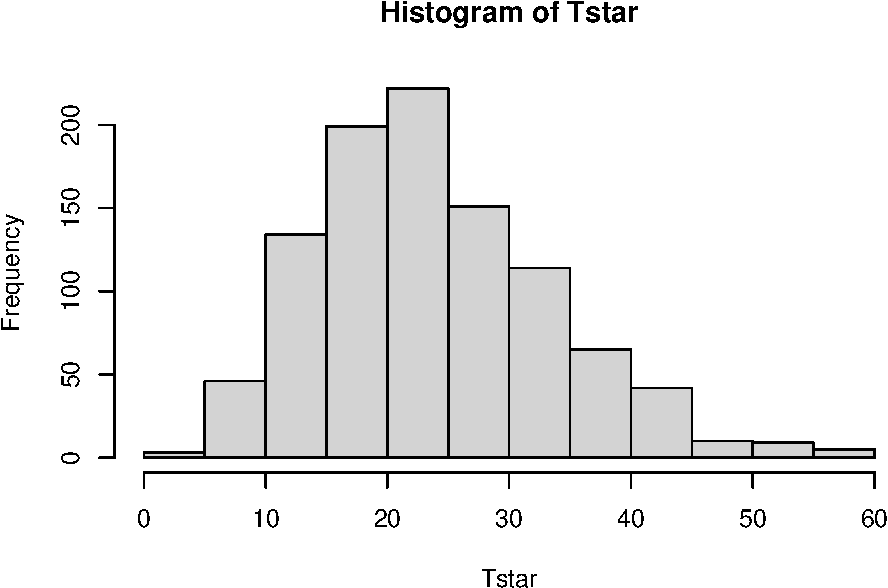
\includegraphics{Assignment2_complete_files/figure-latex/unnamed-chunk-3-1.pdf}

\begin{Shaded}
\begin{Highlighting}[]
\NormalTok{chitest}\SpecialCharTok{$}\NormalTok{p.value}
\end{Highlighting}
\end{Shaded}

\begin{verbatim}
## [1] 0.03642928
\end{verbatim}

\begin{Shaded}
\begin{Highlighting}[]
\NormalTok{chitest}\SpecialCharTok{$}\NormalTok{statistic}
\end{Highlighting}
\end{Shaded}

\begin{verbatim}
## X-squared 
##  6.624765
\end{verbatim}

\begin{Shaded}
\begin{Highlighting}[]
\NormalTok{pl}\OtherTok{=}\FunctionTok{sum}\NormalTok{(Tstar}\SpecialCharTok{\textless{}}\NormalTok{chitest}\SpecialCharTok{$}\NormalTok{statistic)}\SpecialCharTok{/}\NormalTok{B}
\NormalTok{pr}\OtherTok{=}\FunctionTok{sum}\NormalTok{(Tstar}\SpecialCharTok{\textgreater{}}\NormalTok{chitest}\SpecialCharTok{$}\NormalTok{statistic)}\SpecialCharTok{/}\NormalTok{B}
\NormalTok{pl}
\end{Highlighting}
\end{Shaded}

\begin{verbatim}
## [1] 0.011
\end{verbatim}

\begin{Shaded}
\begin{Highlighting}[]
\NormalTok{pr}
\end{Highlighting}
\end{Shaded}

\begin{verbatim}
## [1] 0.989
\end{verbatim}

\begin{Shaded}
\begin{Highlighting}[]
\NormalTok{p\_value }\OtherTok{=} \DecValTok{2}\SpecialCharTok{*}\FunctionTok{min}\NormalTok{(pl,pr)}
\NormalTok{p\_value}
\end{Highlighting}
\end{Shaded}

\begin{verbatim}
## [1] 0.022
\end{verbatim}

\hypertarget{c}{%
\subsubsection{1c}\label{c}}

The p-value obtained by the chisquare test for contingency tables is
0.03642928 and that for the permutation test is 0.034 which is slightly
lower but by a negligable amount, making them around the same. This is
what is to be expected as using different permutations does not change
the distribution of the data and the use of the same test statistic in
both test results in a similar outcome.

\hypertarget{section-1}{%
\subsection{2}\label{section-1}}

\begin{Shaded}
\begin{Highlighting}[]
\NormalTok{airpollution }\OtherTok{\textless{}{-}} \FunctionTok{read.csv}\NormalTok{(}\StringTok{"airpollution.txt"}\NormalTok{, }\AttributeTok{sep=}\StringTok{""}\NormalTok{)}
\FunctionTok{View}\NormalTok{(airpollution)}
\end{Highlighting}
\end{Shaded}

\begin{Shaded}
\begin{Highlighting}[]
\FunctionTok{pairs}\NormalTok{(airpollution)}
\end{Highlighting}
\end{Shaded}

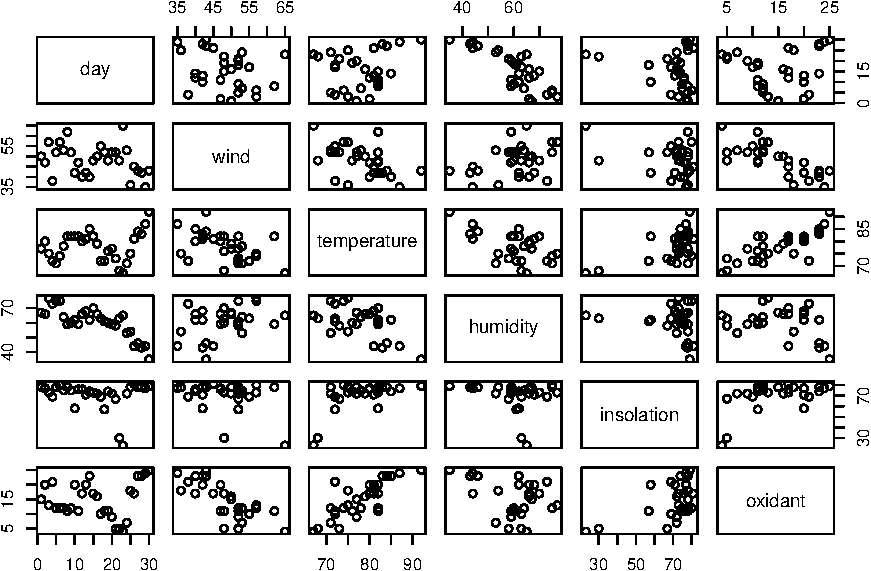
\includegraphics{Assignment2_complete_files/figure-latex/unnamed-chunk-5-1.pdf}

\begin{Shaded}
\begin{Highlighting}[]
\CommentTok{\# temperature and oxidant might have a linear relation}
\end{Highlighting}
\end{Shaded}

\begin{Shaded}
\begin{Highlighting}[]
\NormalTok{dogslr }\OtherTok{=} \FunctionTok{lm}\NormalTok{(oxidant}\SpecialCharTok{\textasciitilde{}}\NormalTok{wind}\SpecialCharTok{+}\NormalTok{temperature}\SpecialCharTok{+}\NormalTok{humidity}\SpecialCharTok{+}\NormalTok{insolation,}\AttributeTok{data=}\NormalTok{airpollution)}
\FunctionTok{summary}\NormalTok{(dogslr)}
\end{Highlighting}
\end{Shaded}

\begin{verbatim}
## 
## Call:
## lm(formula = oxidant ~ wind + temperature + humidity + insolation, 
##     data = airpollution)
## 
## Residuals:
##     Min      1Q  Median      3Q     Max 
## -6.5861 -1.0961  0.3512  1.7570  4.0712 
## 
## Coefficients:
##              Estimate Std. Error t value Pr(>|t|)    
## (Intercept) -15.49370   13.50647  -1.147  0.26219    
## wind         -0.44291    0.08678  -5.104 2.85e-05 ***
## temperature   0.56933    0.13977   4.073  0.00041 ***
## humidity      0.09292    0.06535   1.422  0.16743    
## insolation    0.02275    0.05067   0.449  0.65728    
## ---
## Signif. codes:  0 '***' 0.001 '**' 0.01 '*' 0.05 '.' 0.1 ' ' 1
## 
## Residual standard error: 2.92 on 25 degrees of freedom
## Multiple R-squared:  0.798,  Adjusted R-squared:  0.7657 
## F-statistic: 24.69 on 4 and 25 DF,  p-value: 2.279e-08
\end{verbatim}

p-value for wind and temperature is less than 0.5. Therefore, they are
significant.

Cook's Distance with only significant explanatory variables:

\begin{Shaded}
\begin{Highlighting}[]
\NormalTok{dogsnlm }\OtherTok{=} \FunctionTok{lm}\NormalTok{(oxidant}\SpecialCharTok{\textasciitilde{}}\NormalTok{wind}\SpecialCharTok{+}\NormalTok{temperature,}\AttributeTok{data=}\NormalTok{airpollution)}
\FunctionTok{round}\NormalTok{(}\FunctionTok{cooks.distance}\NormalTok{(dogsnlm),}\DecValTok{2}\NormalTok{)}
\end{Highlighting}
\end{Shaded}

\begin{verbatim}
##    1    2    3    4    5    6    7    8    9   10   11   12   13   14   15   16 
## 0.00 0.02 0.05 0.38 0.02 0.04 0.00 0.00 0.04 0.00 0.09 0.02 0.00 0.01 0.00 0.00 
##   17   18   19   20   21   22   23   24   25   26   27   28   29   30 
## 0.01 0.00 0.01 0.02 0.08 0.21 0.07 0.02 0.00 0.00 0.03 0.03 0.01 0.01
\end{verbatim}

\begin{Shaded}
\begin{Highlighting}[]
\FunctionTok{max}\NormalTok{(}\FunctionTok{round}\NormalTok{(}\FunctionTok{cooks.distance}\NormalTok{(dogsnlm),}\DecValTok{2}\NormalTok{))}
\end{Highlighting}
\end{Shaded}

\begin{verbatim}
## [1] 0.38
\end{verbatim}

No influence point here.

Cook's Distance for entire model :

\begin{Shaded}
\begin{Highlighting}[]
\FunctionTok{round}\NormalTok{(}\FunctionTok{cooks.distance}\NormalTok{(dogslr),}\DecValTok{2}\NormalTok{)}
\end{Highlighting}
\end{Shaded}

\begin{verbatim}
##    1    2    3    4    5    6    7    8    9   10   11   12   13   14   15   16 
## 0.00 0.01 0.03 0.20 0.01 0.02 0.00 0.00 0.03 0.00 0.06 0.04 0.00 0.00 0.01 0.00 
##   17   18   19   20   21   22   23   24   25   26   27   28   29   30 
## 0.01 0.01 0.01 0.02 0.06 0.33 0.83 0.01 0.00 0.00 0.04 0.08 0.00 0.08
\end{verbatim}

\begin{Shaded}
\begin{Highlighting}[]
\FunctionTok{max}\NormalTok{(}\FunctionTok{round}\NormalTok{(}\FunctionTok{cooks.distance}\NormalTok{(dogslr),}\DecValTok{2}\NormalTok{))}
\end{Highlighting}
\end{Shaded}

\begin{verbatim}
## [1] 0.83
\end{verbatim}

\begin{Shaded}
\begin{Highlighting}[]
\FunctionTok{order}\NormalTok{(}\FunctionTok{cooks.distance}\NormalTok{(dogslr))}
\end{Highlighting}
\end{Shaded}

\begin{verbatim}
##  [1]  8 13 25 14 26 10 29  1 16  7 15 17 18 24 19  5  2 20  6  3  9 12 27 11 21
## [26] 28 30  4 22 23
\end{verbatim}

Cook's distance for 23rd data point is close to 1 so it can be an
influence point.

\begin{Shaded}
\begin{Highlighting}[]
\FunctionTok{plot}\NormalTok{(}\DecValTok{1}\SpecialCharTok{:}\DecValTok{30}\NormalTok{,}\FunctionTok{cooks.distance}\NormalTok{(dogslr),}\AttributeTok{type=}\StringTok{"b"}\NormalTok{)}
\end{Highlighting}
\end{Shaded}

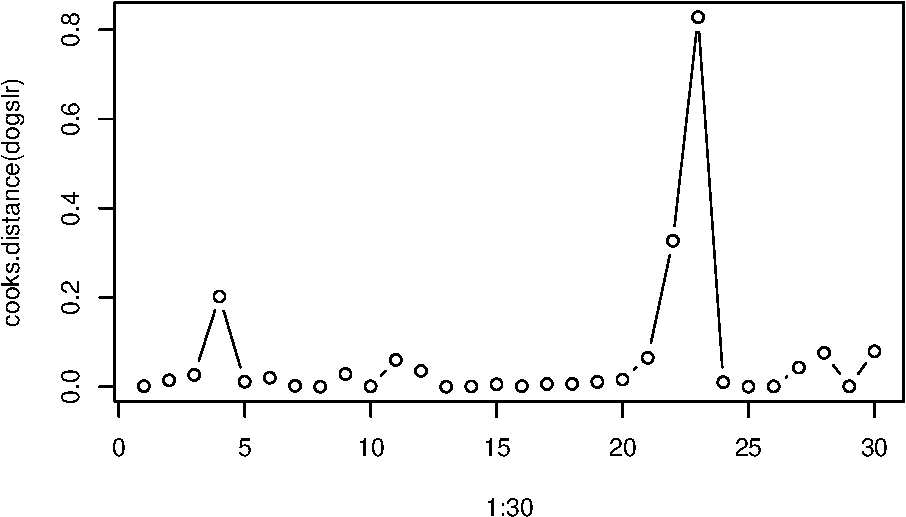
\includegraphics{Assignment2_complete_files/figure-latex/unnamed-chunk-9-1.pdf}
COLLINEARITY:

A.) Pairwise Linear Correlation

\begin{Shaded}
\begin{Highlighting}[]
\FunctionTok{round}\NormalTok{(}\FunctionTok{cor}\NormalTok{(airpollution),}\DecValTok{2}\NormalTok{)}
\end{Highlighting}
\end{Shaded}

\begin{verbatim}
##               day  wind temperature humidity insolation oxidant
## day          1.00 -0.28        0.18    -0.81      -0.16    0.10
## wind        -0.28  1.00       -0.50     0.37      -0.32   -0.77
## temperature  0.18 -0.50        1.00    -0.54       0.57    0.76
## humidity    -0.81  0.37       -0.54     1.00      -0.18   -0.35
## insolation  -0.16 -0.32        0.57    -0.18       1.00    0.51
## oxidant      0.10 -0.77        0.76    -0.35       0.51    1.00
\end{verbatim}

No significant linear correlation

\hypertarget{check-multicolinearity-of-variables}{%
\section{check multicolinearity of variables
:}\label{check-multicolinearity-of-variables}}

\begin{Shaded}
\begin{Highlighting}[]
\CommentTok{\#install.packages("car",dependencies=TRUE)}
\CommentTok{\#library(car)}
\CommentTok{\#vif(dogsnlm)}
\end{Highlighting}
\end{Shaded}

\begin{Shaded}
\begin{Highlighting}[]
\NormalTok{x}\OtherTok{=}\FunctionTok{residuals}\NormalTok{(}\FunctionTok{lm}\NormalTok{(wind}\SpecialCharTok{\textasciitilde{}}\NormalTok{temperature}\SpecialCharTok{+}\NormalTok{humidity}\SpecialCharTok{+}\NormalTok{insolation,}\AttributeTok{data=}\NormalTok{airpollution))}
\NormalTok{y}\OtherTok{=}\FunctionTok{residuals}\NormalTok{(}\FunctionTok{lm}\NormalTok{(oxidant}\SpecialCharTok{\textasciitilde{}}\NormalTok{temperature}\SpecialCharTok{+}\NormalTok{humidity}\SpecialCharTok{+}\NormalTok{insolation,}\AttributeTok{data=}\NormalTok{airpollution))}
\FunctionTok{plot}\NormalTok{(x,y,}\AttributeTok{main=}\StringTok{"Added variable plot for wind"}\NormalTok{, }\AttributeTok{xlab=}\StringTok{"residual of wind"}\NormalTok{,}\AttributeTok{ylab=}\StringTok{"residual of oxidant"}\NormalTok{)}
\end{Highlighting}
\end{Shaded}

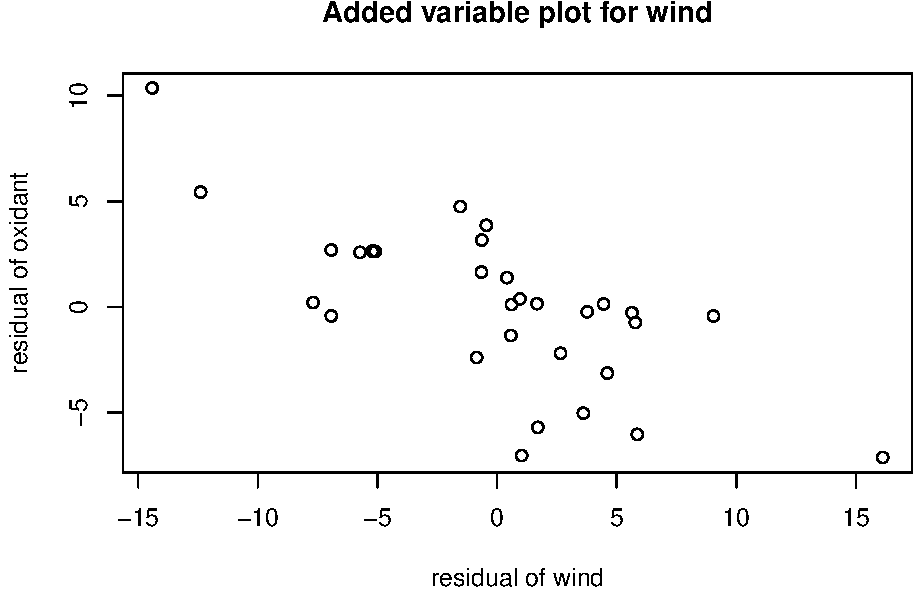
\includegraphics{Assignment2_complete_files/figure-latex/unnamed-chunk-12-1.pdf}

\begin{Shaded}
\begin{Highlighting}[]
\NormalTok{x\_new}\OtherTok{=}\FunctionTok{residuals}\NormalTok{(}\FunctionTok{lm}\NormalTok{(wind}\SpecialCharTok{\textasciitilde{}}\NormalTok{temperature,}\AttributeTok{data=}\NormalTok{airpollution))}
\NormalTok{y\_new}\OtherTok{=}\FunctionTok{residuals}\NormalTok{(}\FunctionTok{lm}\NormalTok{(oxidant}\SpecialCharTok{\textasciitilde{}}\NormalTok{temperature,}\AttributeTok{data=}\NormalTok{airpollution))}
\FunctionTok{summary}\NormalTok{(}\FunctionTok{lm}\NormalTok{(y\_new}\SpecialCharTok{\textasciitilde{}}\NormalTok{x\_new))}
\end{Highlighting}
\end{Shaded}

\begin{verbatim}
## 
## Call:
## lm(formula = y_new ~ x_new)
## 
## Residuals:
##     Min      1Q  Median      3Q     Max 
## -6.3939 -1.8608  0.5826  1.9461  4.9661 
## 
## Coefficients:
##               Estimate Std. Error t value Pr(>|t|)    
## (Intercept)  6.968e-17  5.288e-01   0.000        1    
## x_new       -4.271e-01  8.489e-02  -5.031 2.55e-05 ***
## ---
## Signif. codes:  0 '***' 0.001 '**' 0.01 '*' 0.05 '.' 0.1 ' ' 1
## 
## Residual standard error: 2.896 on 28 degrees of freedom
## Multiple R-squared:  0.4748, Adjusted R-squared:  0.456 
## F-statistic: 25.31 on 1 and 28 DF,  p-value: 2.549e-05
\end{verbatim}

\begin{Shaded}
\begin{Highlighting}[]
\FunctionTok{summary}\NormalTok{(dogsnlm)}
\end{Highlighting}
\end{Shaded}

\begin{verbatim}
## 
## Call:
## lm(formula = oxidant ~ wind + temperature, data = airpollution)
## 
## Residuals:
##     Min      1Q  Median      3Q     Max 
## -6.3939 -1.8608  0.5826  1.9461  4.9661 
## 
## Coefficients:
##             Estimate Std. Error t value Pr(>|t|)    
## (Intercept) -5.20334   11.11810  -0.468    0.644    
## wind        -0.42706    0.08645  -4.940 3.58e-05 ***
## temperature  0.52035    0.10813   4.812 5.05e-05 ***
## ---
## Signif. codes:  0 '***' 0.001 '**' 0.01 '*' 0.05 '.' 0.1 ' ' 1
## 
## Residual standard error: 2.95 on 27 degrees of freedom
## Multiple R-squared:  0.7773, Adjusted R-squared:  0.7608 
## F-statistic: 47.12 on 2 and 27 DF,  p-value: 1.563e-09
\end{verbatim}

Step-up model:

\begin{Shaded}
\begin{Highlighting}[]
\FunctionTok{summary}\NormalTok{(}\FunctionTok{lm}\NormalTok{(oxidant}\SpecialCharTok{\textasciitilde{}}\NormalTok{wind,}\AttributeTok{data=}\NormalTok{airpollution))}
\end{Highlighting}
\end{Shaded}

\begin{verbatim}
## 
## Call:
## lm(formula = oxidant ~ wind, data = airpollution)
## 
## Residuals:
##     Min      1Q  Median      3Q     Max 
## -9.9266 -2.5923  0.2065  2.6636  6.9077 
## 
## Coefficients:
##             Estimate Std. Error t value Pr(>|t|)    
## (Intercept)  45.3171     4.8976   9.253 5.19e-10 ***
## wind         -0.6331     0.1005  -6.300 8.20e-07 ***
## ---
## Signif. codes:  0 '***' 0.001 '**' 0.01 '*' 0.05 '.' 0.1 ' ' 1
## 
## Residual standard error: 3.948 on 28 degrees of freedom
## Multiple R-squared:  0.5863, Adjusted R-squared:  0.5715 
## F-statistic: 39.68 on 1 and 28 DF,  p-value: 8.205e-07
\end{verbatim}

\begin{Shaded}
\begin{Highlighting}[]
\FunctionTok{summary}\NormalTok{(}\FunctionTok{lm}\NormalTok{(oxidant}\SpecialCharTok{\textasciitilde{}}\NormalTok{temperature,}\AttributeTok{data=}\NormalTok{airpollution))}
\end{Highlighting}
\end{Shaded}

\begin{verbatim}
## 
## Call:
## lm(formula = oxidant ~ temperature, data = airpollution)
## 
## Residuals:
##     Min      1Q  Median      3Q     Max 
## -6.9400 -2.2138  0.3775  2.5550 10.9099 
## 
## Coefficients:
##             Estimate Std. Error t value Pr(>|t|)    
## (Intercept) -46.4292     9.9542  -4.664 6.94e-05 ***
## temperature   0.7850     0.1273   6.168 1.17e-06 ***
## ---
## Signif. codes:  0 '***' 0.001 '**' 0.01 '*' 0.05 '.' 0.1 ' ' 1
## 
## Residual standard error: 3.997 on 28 degrees of freedom
## Multiple R-squared:  0.576,  Adjusted R-squared:  0.5609 
## F-statistic: 38.04 on 1 and 28 DF,  p-value: 1.167e-06
\end{verbatim}

\begin{Shaded}
\begin{Highlighting}[]
\FunctionTok{summary}\NormalTok{(}\FunctionTok{lm}\NormalTok{(oxidant}\SpecialCharTok{\textasciitilde{}}\NormalTok{humidity,}\AttributeTok{data=}\NormalTok{airpollution))}
\end{Highlighting}
\end{Shaded}

\begin{verbatim}
## 
## Call:
## lm(formula = oxidant ~ humidity, data = airpollution)
## 
## Residuals:
##      Min       1Q   Median       3Q      Max 
## -10.3358  -4.0749   0.8782   4.7800   8.7957 
## 
## Coefficients:
##             Estimate Std. Error t value Pr(>|t|)    
## (Intercept)  27.4446     6.4368   4.264 0.000206 ***
## humidity     -0.2088     0.1049  -1.991 0.056317 .  
## ---
## Signif. codes:  0 '***' 0.001 '**' 0.01 '*' 0.05 '.' 0.1 ' ' 1
## 
## Residual standard error: 5.745 on 28 degrees of freedom
## Multiple R-squared:  0.124,  Adjusted R-squared:  0.09273 
## F-statistic: 3.964 on 1 and 28 DF,  p-value: 0.05632
\end{verbatim}

\begin{Shaded}
\begin{Highlighting}[]
\FunctionTok{summary}\NormalTok{(}\FunctionTok{lm}\NormalTok{(oxidant}\SpecialCharTok{\textasciitilde{}}\NormalTok{insolation,}\AttributeTok{data=}\NormalTok{airpollution))}
\end{Highlighting}
\end{Shaded}

\begin{verbatim}
## 
## Call:
## lm(formula = oxidant ~ insolation, data = airpollution)
## 
## Residuals:
##     Min      1Q  Median      3Q     Max 
## -8.9723 -4.4841 -0.3281  4.7631  8.2686 
## 
## Coefficients:
##             Estimate Std. Error t value Pr(>|t|)   
## (Intercept) -1.43279    5.32967  -0.269  0.79003   
## insolation   0.22993    0.07424   3.097  0.00441 **
## ---
## Signif. codes:  0 '***' 0.001 '**' 0.01 '*' 0.05 '.' 0.1 ' ' 1
## 
## Residual standard error: 5.297 on 28 degrees of freedom
## Multiple R-squared:  0.2552, Adjusted R-squared:  0.2286 
## F-statistic: 9.592 on 1 and 28 DF,  p-value: 0.004411
\end{verbatim}

wind has the highest R-square value and a p-value \textless{} 0.05 .
Therefore, we add this explanatory variable to or model.

\begin{Shaded}
\begin{Highlighting}[]
\FunctionTok{summary}\NormalTok{(}\FunctionTok{lm}\NormalTok{(oxidant}\SpecialCharTok{\textasciitilde{}}\NormalTok{wind}\SpecialCharTok{+}\NormalTok{temperature,}\AttributeTok{data=}\NormalTok{airpollution))}
\end{Highlighting}
\end{Shaded}

\begin{verbatim}
## 
## Call:
## lm(formula = oxidant ~ wind + temperature, data = airpollution)
## 
## Residuals:
##     Min      1Q  Median      3Q     Max 
## -6.3939 -1.8608  0.5826  1.9461  4.9661 
## 
## Coefficients:
##             Estimate Std. Error t value Pr(>|t|)    
## (Intercept) -5.20334   11.11810  -0.468    0.644    
## wind        -0.42706    0.08645  -4.940 3.58e-05 ***
## temperature  0.52035    0.10813   4.812 5.05e-05 ***
## ---
## Signif. codes:  0 '***' 0.001 '**' 0.01 '*' 0.05 '.' 0.1 ' ' 1
## 
## Residual standard error: 2.95 on 27 degrees of freedom
## Multiple R-squared:  0.7773, Adjusted R-squared:  0.7608 
## F-statistic: 47.12 on 2 and 27 DF,  p-value: 1.563e-09
\end{verbatim}

\begin{Shaded}
\begin{Highlighting}[]
\FunctionTok{summary}\NormalTok{(}\FunctionTok{lm}\NormalTok{(oxidant}\SpecialCharTok{\textasciitilde{}}\NormalTok{wind}\SpecialCharTok{+}\NormalTok{humidity,}\AttributeTok{data=}\NormalTok{airpollution))}
\end{Highlighting}
\end{Shaded}

\begin{verbatim}
## 
## Call:
## lm(formula = oxidant ~ wind + humidity, data = airpollution)
## 
## Residuals:
##     Min      1Q  Median      3Q     Max 
## -9.8120 -2.2808  0.3433  3.0476  5.8757 
## 
## Coefficients:
##             Estimate Std. Error t value Pr(>|t|)    
## (Intercept) 46.91570    5.68573   8.251 7.38e-09 ***
## wind        -0.60955    0.10971  -5.556 6.86e-06 ***
## humidity    -0.04516    0.07866  -0.574    0.571    
## ---
## Signif. codes:  0 '***' 0.001 '**' 0.01 '*' 0.05 '.' 0.1 ' ' 1
## 
## Residual standard error: 3.996 on 27 degrees of freedom
## Multiple R-squared:  0.5913, Adjusted R-squared:  0.561 
## F-statistic: 19.53 on 2 and 27 DF,  p-value: 5.674e-06
\end{verbatim}

\begin{Shaded}
\begin{Highlighting}[]
\FunctionTok{summary}\NormalTok{(}\FunctionTok{lm}\NormalTok{(oxidant}\SpecialCharTok{\textasciitilde{}}\NormalTok{wind}\SpecialCharTok{+}\NormalTok{insolation,}\AttributeTok{data=}\NormalTok{airpollution))}
\end{Highlighting}
\end{Shaded}

\begin{verbatim}
## 
## Call:
## lm(formula = oxidant ~ wind + insolation, data = airpollution)
## 
## Residuals:
##     Min      1Q  Median      3Q     Max 
## -7.2119 -2.7198  0.4815  2.8733  6.2012 
## 
## Coefficients:
##             Estimate Std. Error t value Pr(>|t|)    
## (Intercept) 32.32615    6.97098   4.637 8.07e-05 ***
## wind        -0.55639    0.09778  -5.690 4.81e-06 ***
## insolation   0.13161    0.05383   2.445   0.0213 *  
## ---
## Signif. codes:  0 '***' 0.001 '**' 0.01 '*' 0.05 '.' 0.1 ' ' 1
## 
## Residual standard error: 3.638 on 27 degrees of freedom
## Multiple R-squared:  0.6613, Adjusted R-squared:  0.6362 
## F-statistic: 26.36 on 2 and 27 DF,  p-value: 4.491e-07
\end{verbatim}

Next we add temperature. It has the highest R square value and the
variable is significant.

\begin{Shaded}
\begin{Highlighting}[]
\FunctionTok{summary}\NormalTok{(}\FunctionTok{lm}\NormalTok{(oxidant}\SpecialCharTok{\textasciitilde{}}\NormalTok{wind}\SpecialCharTok{+}\NormalTok{temperature}\SpecialCharTok{+}\NormalTok{humidity,}\AttributeTok{data=}\NormalTok{airpollution))}
\end{Highlighting}
\end{Shaded}

\begin{verbatim}
## 
## Call:
## lm(formula = oxidant ~ wind + temperature + humidity, data = airpollution)
## 
## Residuals:
##     Min      1Q  Median      3Q     Max 
## -6.5887 -1.1686  0.1978  1.9004  4.1544 
## 
## Coefficients:
##              Estimate Std. Error t value Pr(>|t|)    
## (Intercept) -16.60697   13.07154  -1.270    0.215    
## wind         -0.44620    0.08513  -5.241 1.78e-05 ***
## temperature   0.60190    0.11764   5.117 2.47e-05 ***
## humidity      0.09850    0.06316   1.559    0.131    
## ---
## Signif. codes:  0 '***' 0.001 '**' 0.01 '*' 0.05 '.' 0.1 ' ' 1
## 
## Residual standard error: 2.874 on 26 degrees of freedom
## Multiple R-squared:  0.7964, Adjusted R-squared:  0.7729 
## F-statistic: 33.89 on 3 and 26 DF,  p-value: 3.904e-09
\end{verbatim}

\begin{Shaded}
\begin{Highlighting}[]
\FunctionTok{summary}\NormalTok{(}\FunctionTok{lm}\NormalTok{(oxidant}\SpecialCharTok{\textasciitilde{}}\NormalTok{wind}\SpecialCharTok{+}\NormalTok{temperature}\SpecialCharTok{+}\NormalTok{insolation,}\AttributeTok{data=}\NormalTok{airpollution))}
\end{Highlighting}
\end{Shaded}

\begin{verbatim}
## 
## Call:
## lm(formula = oxidant ~ wind + temperature + insolation, data = airpollution)
## 
## Residuals:
##    Min     1Q Median     3Q    Max 
## -6.407 -2.056  1.012  1.760  4.792 
## 
## Coefficients:
##             Estimate Std. Error t value Pr(>|t|)    
## (Intercept) -4.45496   11.26714  -0.395 0.695778    
## wind        -0.42353    0.08737  -4.848 5.02e-05 ***
## temperature  0.47558    0.12564   3.785 0.000816 ***
## insolation   0.03646    0.05071   0.719 0.478636    
## ---
## Signif. codes:  0 '***' 0.001 '**' 0.01 '*' 0.05 '.' 0.1 ' ' 1
## 
## Residual standard error: 2.976 on 26 degrees of freedom
## Multiple R-squared:  0.7816, Adjusted R-squared:  0.7565 
## F-statistic: 31.02 on 3 and 26 DF,  p-value: 9.583e-09
\end{verbatim}

None of the other explanatory variables - humidity and insolation are
significant. Therefore our linear model has only two explanatory
variables - wind and temperature.

\begin{Shaded}
\begin{Highlighting}[]
\NormalTok{lm\_up }\OtherTok{=} \FunctionTok{lm}\NormalTok{(oxidant}\SpecialCharTok{\textasciitilde{}}\NormalTok{wind}\SpecialCharTok{+}\NormalTok{temperature,}\AttributeTok{data=}\NormalTok{airpollution)}
\FunctionTok{summary}\NormalTok{(lm\_up)}
\end{Highlighting}
\end{Shaded}

\begin{verbatim}
## 
## Call:
## lm(formula = oxidant ~ wind + temperature, data = airpollution)
## 
## Residuals:
##     Min      1Q  Median      3Q     Max 
## -6.3939 -1.8608  0.5826  1.9461  4.9661 
## 
## Coefficients:
##             Estimate Std. Error t value Pr(>|t|)    
## (Intercept) -5.20334   11.11810  -0.468    0.644    
## wind        -0.42706    0.08645  -4.940 3.58e-05 ***
## temperature  0.52035    0.10813   4.812 5.05e-05 ***
## ---
## Signif. codes:  0 '***' 0.001 '**' 0.01 '*' 0.05 '.' 0.1 ' ' 1
## 
## Residual standard error: 2.95 on 27 degrees of freedom
## Multiple R-squared:  0.7773, Adjusted R-squared:  0.7608 
## F-statistic: 47.12 on 2 and 27 DF,  p-value: 1.563e-09
\end{verbatim}

oxidant = -5.20334 + (-0.42706)*wind + (0.52035)temperature + error

STEP DOWN :

\begin{Shaded}
\begin{Highlighting}[]
\FunctionTok{summary}\NormalTok{(}\FunctionTok{lm}\NormalTok{(oxidant}\SpecialCharTok{\textasciitilde{}}\NormalTok{wind}\SpecialCharTok{+}\NormalTok{temperature}\SpecialCharTok{+}\NormalTok{humidity}\SpecialCharTok{+}\NormalTok{insolation,}\AttributeTok{data=}\NormalTok{airpollution))}
\end{Highlighting}
\end{Shaded}

\begin{verbatim}
## 
## Call:
## lm(formula = oxidant ~ wind + temperature + humidity + insolation, 
##     data = airpollution)
## 
## Residuals:
##     Min      1Q  Median      3Q     Max 
## -6.5861 -1.0961  0.3512  1.7570  4.0712 
## 
## Coefficients:
##              Estimate Std. Error t value Pr(>|t|)    
## (Intercept) -15.49370   13.50647  -1.147  0.26219    
## wind         -0.44291    0.08678  -5.104 2.85e-05 ***
## temperature   0.56933    0.13977   4.073  0.00041 ***
## humidity      0.09292    0.06535   1.422  0.16743    
## insolation    0.02275    0.05067   0.449  0.65728    
## ---
## Signif. codes:  0 '***' 0.001 '**' 0.01 '*' 0.05 '.' 0.1 ' ' 1
## 
## Residual standard error: 2.92 on 25 degrees of freedom
## Multiple R-squared:  0.798,  Adjusted R-squared:  0.7657 
## F-statistic: 24.69 on 4 and 25 DF,  p-value: 2.279e-08
\end{verbatim}

Insolation has the largest p-value and it is greater than 0.05.
Therefore, we remove Insolation variable from the linear model.

\begin{Shaded}
\begin{Highlighting}[]
\FunctionTok{summary}\NormalTok{(}\FunctionTok{lm}\NormalTok{(oxidant}\SpecialCharTok{\textasciitilde{}}\NormalTok{wind}\SpecialCharTok{+}\NormalTok{temperature}\SpecialCharTok{+}\NormalTok{humidity,}\AttributeTok{data=}\NormalTok{airpollution))}
\end{Highlighting}
\end{Shaded}

\begin{verbatim}
## 
## Call:
## lm(formula = oxidant ~ wind + temperature + humidity, data = airpollution)
## 
## Residuals:
##     Min      1Q  Median      3Q     Max 
## -6.5887 -1.1686  0.1978  1.9004  4.1544 
## 
## Coefficients:
##              Estimate Std. Error t value Pr(>|t|)    
## (Intercept) -16.60697   13.07154  -1.270    0.215    
## wind         -0.44620    0.08513  -5.241 1.78e-05 ***
## temperature   0.60190    0.11764   5.117 2.47e-05 ***
## humidity      0.09850    0.06316   1.559    0.131    
## ---
## Signif. codes:  0 '***' 0.001 '**' 0.01 '*' 0.05 '.' 0.1 ' ' 1
## 
## Residual standard error: 2.874 on 26 degrees of freedom
## Multiple R-squared:  0.7964, Adjusted R-squared:  0.7729 
## F-statistic: 33.89 on 3 and 26 DF,  p-value: 3.904e-09
\end{verbatim}

Largest p-value of humidity is \textgreater{} 0.05. Therefore, we remove
humidity from the model.

\begin{Shaded}
\begin{Highlighting}[]
\FunctionTok{summary}\NormalTok{(}\FunctionTok{lm}\NormalTok{(oxidant}\SpecialCharTok{\textasciitilde{}}\NormalTok{wind}\SpecialCharTok{+}\NormalTok{temperature,}\AttributeTok{data=}\NormalTok{airpollution))}
\end{Highlighting}
\end{Shaded}

\begin{verbatim}
## 
## Call:
## lm(formula = oxidant ~ wind + temperature, data = airpollution)
## 
## Residuals:
##     Min      1Q  Median      3Q     Max 
## -6.3939 -1.8608  0.5826  1.9461  4.9661 
## 
## Coefficients:
##             Estimate Std. Error t value Pr(>|t|)    
## (Intercept) -5.20334   11.11810  -0.468    0.644    
## wind        -0.42706    0.08645  -4.940 3.58e-05 ***
## temperature  0.52035    0.10813   4.812 5.05e-05 ***
## ---
## Signif. codes:  0 '***' 0.001 '**' 0.01 '*' 0.05 '.' 0.1 ' ' 1
## 
## Residual standard error: 2.95 on 27 degrees of freedom
## Multiple R-squared:  0.7773, Adjusted R-squared:  0.7608 
## F-statistic: 47.12 on 2 and 27 DF,  p-value: 1.563e-09
\end{verbatim}

oxidant = -5.20334 + (-0.42706)*wind + (0.52035)temperature + error

We get the same model from both step up and step down approaches.
Therefore, we don't need to compare the models.

\begin{Shaded}
\begin{Highlighting}[]
\NormalTok{linear\_model }\OtherTok{=} \FunctionTok{lm}\NormalTok{(oxidant}\SpecialCharTok{\textasciitilde{}}\NormalTok{wind}\SpecialCharTok{+}\NormalTok{temperature,}\AttributeTok{data=}\NormalTok{airpollution)}
\NormalTok{x\_newdata }\OtherTok{=} \FunctionTok{data.frame}\NormalTok{(}\AttributeTok{wind=}\DecValTok{33}\NormalTok{,}\AttributeTok{temperature=}\DecValTok{54}\NormalTok{)}
\FunctionTok{predict}\NormalTok{(linear\_model,x\_newdata,}\AttributeTok{interval=}\StringTok{"confidence"}\NormalTok{)}
\end{Highlighting}
\end{Shaded}

\begin{verbatim}
##       fit      lwr      upr
## 1 8.80281 1.656548 15.94907
\end{verbatim}

\begin{Shaded}
\begin{Highlighting}[]
\FunctionTok{predict}\NormalTok{(linear\_model,x\_newdata,}\AttributeTok{interval=}\StringTok{"prediction"}\NormalTok{)}
\end{Highlighting}
\end{Shaded}

\begin{verbatim}
##       fit        lwr      upr
## 1 8.80281 -0.5617877 18.16741
\end{verbatim}

\begin{Shaded}
\begin{Highlighting}[]
\DocumentationTok{\#\# what does negative value imply over here ?}
\end{Highlighting}
\end{Shaded}

\hypertarget{section-2}{%
\subsection{3}\label{section-2}}

Load fruitflies.txt and add loglongevity column

\begin{Shaded}
\begin{Highlighting}[]
\NormalTok{fruitflies }\OtherTok{=} \FunctionTok{read.csv}\NormalTok{(}\StringTok{"fruitflies.txt"}\NormalTok{, }\AttributeTok{sep=}\StringTok{""}\NormalTok{)}
\NormalTok{fruitflies }\OtherTok{=}\NormalTok{ fruitflies[}\FunctionTok{sample}\NormalTok{(}\FunctionTok{nrow}\NormalTok{(fruitflies)),]}
\NormalTok{loglong }\OtherTok{=} \FunctionTok{log}\NormalTok{(fruitflies[}\StringTok{"longevity"}\NormalTok{])}
\NormalTok{fruitflies[}\StringTok{\textquotesingle{}loglongevity\textquotesingle{}}\NormalTok{] }\OtherTok{=}\NormalTok{ loglong}
\end{Highlighting}
\end{Shaded}

\hypertarget{a.-1}{%
\subsubsection{3a.}\label{a.-1}}

We want to know if there is a statistically significant difference
between three groups, based on one variable (log longevity). Therefore,
we use a one-way ANOVA test.

Firs, we create an informative graph, plotting the thorax variable
against the log longevity variable for each type of activity

\begin{Shaded}
\begin{Highlighting}[]
\NormalTok{high }\OtherTok{=} \FunctionTok{subset}\NormalTok{(fruitflies, activity }\SpecialCharTok{==} \StringTok{\textquotesingle{}high\textquotesingle{}}\NormalTok{)}
\NormalTok{low }\OtherTok{=} \FunctionTok{subset}\NormalTok{(fruitflies, activity }\SpecialCharTok{==} \StringTok{\textquotesingle{}low\textquotesingle{}}\NormalTok{)}
\NormalTok{isolated }\OtherTok{=} \FunctionTok{subset}\NormalTok{(fruitflies, activity }\SpecialCharTok{==} \StringTok{\textquotesingle{}isolated\textquotesingle{}}\NormalTok{)}

\FunctionTok{plot}\NormalTok{(high}\SpecialCharTok{$}\NormalTok{thorax, high}\SpecialCharTok{$}\NormalTok{longevity, }\AttributeTok{col=}\StringTok{\textquotesingle{}blue\textquotesingle{}}\NormalTok{, }\AttributeTok{pch=}\DecValTok{20}\NormalTok{)}
\FunctionTok{points}\NormalTok{(low}\SpecialCharTok{$}\NormalTok{thorax, low}\SpecialCharTok{$}\NormalTok{longevity, }\AttributeTok{col=}\StringTok{\textquotesingle{}red\textquotesingle{}}\NormalTok{, }\AttributeTok{pch=}\DecValTok{20}\NormalTok{)}
\FunctionTok{points}\NormalTok{(isolated}\SpecialCharTok{$}\NormalTok{thorax, isolated}\SpecialCharTok{$}\NormalTok{longevity, }\AttributeTok{col=}\StringTok{\textquotesingle{}green\textquotesingle{}}\NormalTok{, }\AttributeTok{pch=}\DecValTok{20}\NormalTok{)}
\end{Highlighting}
\end{Shaded}

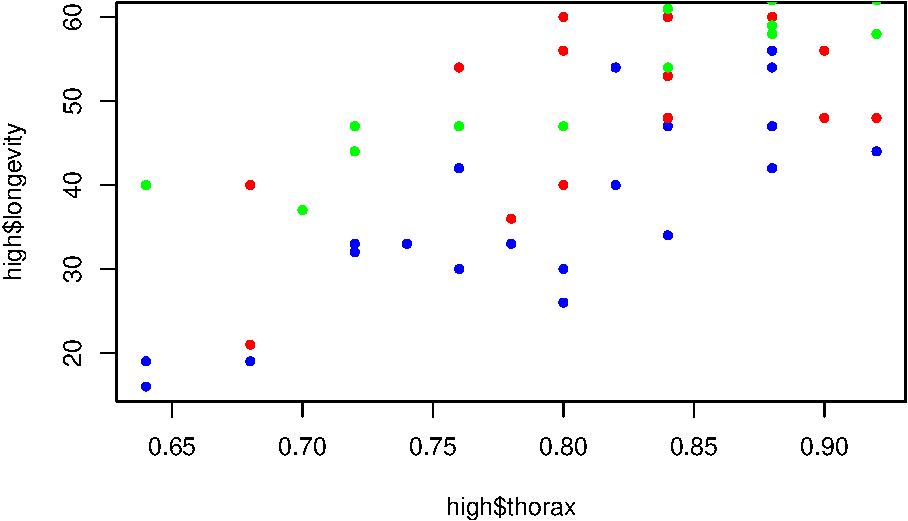
\includegraphics{Assignment2_complete_files/figure-latex/unnamed-chunk-23-1.pdf}

Then, we perform the anova test:

\begin{Shaded}
\begin{Highlighting}[]
\NormalTok{fruitflies\_model }\OtherTok{\textless{}{-}} \FunctionTok{aov}\NormalTok{(loglongevity }\SpecialCharTok{\textasciitilde{}}\NormalTok{ activity, }\AttributeTok{data=}\NormalTok{fruitflies)}
\NormalTok{fruitflies\_model}
\end{Highlighting}
\end{Shaded}

\begin{verbatim}
## Call:
##    aov(formula = loglongevity ~ activity, data = fruitflies)
## 
## Terms:
##                 activity Residuals
## Sum of Squares  3.666493  6.796579
## Deg. of Freedom        2        72
## 
## Residual standard error: 0.3072408
## Estimated effects may be unbalanced
\end{verbatim}

\begin{Shaded}
\begin{Highlighting}[]
\FunctionTok{summary}\NormalTok{(fruitflies\_model)}
\end{Highlighting}
\end{Shaded}

\begin{verbatim}
##             Df Sum Sq Mean Sq F value  Pr(>F)    
## activity     2  3.666  1.8332   19.42 1.8e-07 ***
## Residuals   72  6.797  0.0944                    
## ---
## Signif. codes:  0 '***' 0.001 '**' 0.01 '*' 0.05 '.' 0.1 ' ' 1
\end{verbatim}

We can see that the p-value for activity is well below 0.05. Therefore,
the sexual activity \emph{influences} the longevity.

To estimate the longevities for each of the three conditions, we take
the means:

\begin{Shaded}
\begin{Highlighting}[]
\FunctionTok{mean}\NormalTok{(high}\SpecialCharTok{$}\NormalTok{longevity)}
\end{Highlighting}
\end{Shaded}

\begin{verbatim}
## [1] 38.72
\end{verbatim}

\begin{Shaded}
\begin{Highlighting}[]
\FunctionTok{mean}\NormalTok{(low}\SpecialCharTok{$}\NormalTok{longevity)}
\end{Highlighting}
\end{Shaded}

\begin{verbatim}
## [1] 56.76
\end{verbatim}

\begin{Shaded}
\begin{Highlighting}[]
\FunctionTok{mean}\NormalTok{(isolated}\SpecialCharTok{$}\NormalTok{longevity)}
\end{Highlighting}
\end{Shaded}

\begin{verbatim}
## [1] 63.56
\end{verbatim}

Therefore, the longevity for \emph{high activity} is 38.72, for
\emph{low activity} is 56.76, for \emph{isolated activity} is 63.56

This means that the higher the sexual activity, the shorter the
fruitflies live.

\hypertarget{b.-1}{%
\subsubsection{3b.}\label{b.-1}}

We now include the thorax variable, which is a numerical variable. That
means we now have a factor variable, a numerical variable and a
numerical outcome, which means that an ANCOVA-test is appropriate. We
use the drop1 function to make sure the result is correct even if the
ANCOVA test is not balanced

\begin{Shaded}
\begin{Highlighting}[]
\NormalTok{fruitflies}\SpecialCharTok{$}\NormalTok{activity }\OtherTok{=} \FunctionTok{as.factor}\NormalTok{(fruitflies}\SpecialCharTok{$}\NormalTok{activity)}
\NormalTok{fruitflies\_model2 }\OtherTok{=} \FunctionTok{drop1}\NormalTok{(}\FunctionTok{lm}\NormalTok{(loglongevity }\SpecialCharTok{\textasciitilde{}}\NormalTok{ activity }\SpecialCharTok{+}\NormalTok{ thorax, }\AttributeTok{data=}\NormalTok{fruitflies), }\AttributeTok{test=}\StringTok{"F"}\NormalTok{)}
\NormalTok{fruitflies\_model2}
\end{Highlighting}
\end{Shaded}

\begin{verbatim}
## Single term deletions
## 
## Model:
## loglongevity ~ activity + thorax
##          Df Sum of Sq    RSS     AIC F value    Pr(>F)    
## <none>                2.9180 -235.50                      
## activity  2    2.1129 5.0309 -198.64  25.705 4.000e-09 ***
## thorax    1    3.8786 6.7966 -174.08  94.374 1.139e-14 ***
## ---
## Signif. codes:  0 '***' 0.001 '**' 0.01 '*' 0.05 '.' 0.1 ' ' 1
\end{verbatim}

\begin{Shaded}
\begin{Highlighting}[]
\FunctionTok{summary}\NormalTok{(fruitflies\_model2)}
\end{Highlighting}
\end{Shaded}

\begin{verbatim}
##        Df         Sum of Sq          RSS             AIC        
##  Min.   :1.00   Min.   :2.113   Min.   :2.918   Min.   :-235.5  
##  1st Qu.:1.25   1st Qu.:2.554   1st Qu.:3.974   1st Qu.:-217.1  
##  Median :1.50   Median :2.996   Median :5.031   Median :-198.6  
##  Mean   :1.50   Mean   :2.996   Mean   :4.915   Mean   :-202.7  
##  3rd Qu.:1.75   3rd Qu.:3.437   3rd Qu.:5.914   3rd Qu.:-186.4  
##  Max.   :2.00   Max.   :3.879   Max.   :6.797   Max.   :-174.1  
##  NA's   :1      NA's   :1                                       
##     F value          Pr(>F) 
##  Min.   :25.71   Min.   :0  
##  1st Qu.:42.87   1st Qu.:0  
##  Median :60.04   Median :0  
##  Mean   :60.04   Mean   :0  
##  3rd Qu.:77.21   3rd Qu.:0  
##  Max.   :94.37   Max.   :0  
##  NA's   :1       NA's   :1
\end{verbatim}

From the p-values, we can see that both the thorax variable and the
activity variable influence the longevity, as these p-values are both
well below 0.05.

If we take the maximum and minimum thorax lengths, we get the following
thorax lengths and longevities:

\begin{Shaded}
\begin{Highlighting}[]
\NormalTok{max\_thorax }\OtherTok{=} \FunctionTok{max}\NormalTok{(fruitflies[}\StringTok{\textquotesingle{}thorax\textquotesingle{}}\NormalTok{])}
\NormalTok{min\_thorax }\OtherTok{=} \FunctionTok{min}\NormalTok{(fruitflies[}\StringTok{\textquotesingle{}thorax\textquotesingle{}}\NormalTok{])}
\NormalTok{max\_thorax\_ff }\OtherTok{=} \FunctionTok{subset}\NormalTok{(fruitflies, thorax }\SpecialCharTok{==}\NormalTok{ max\_thorax)}
\NormalTok{min\_thorax\_ff }\OtherTok{=} \FunctionTok{subset}\NormalTok{(fruitflies, thorax }\SpecialCharTok{==}\NormalTok{ min\_thorax)}

\NormalTok{high\_max }\OtherTok{=} \FunctionTok{subset}\NormalTok{(high, thorax }\SpecialCharTok{==} \FunctionTok{max}\NormalTok{(high[}\StringTok{\textquotesingle{}thorax\textquotesingle{}}\NormalTok{]))}
\NormalTok{high\_min }\OtherTok{=} \FunctionTok{subset}\NormalTok{(high, thorax }\SpecialCharTok{==} \FunctionTok{min}\NormalTok{(high[}\StringTok{\textquotesingle{}thorax\textquotesingle{}}\NormalTok{]))}
\NormalTok{low\_max }\OtherTok{=} \FunctionTok{subset}\NormalTok{(low, thorax }\SpecialCharTok{==} \FunctionTok{max}\NormalTok{(low[}\StringTok{\textquotesingle{}thorax\textquotesingle{}}\NormalTok{]))}
\NormalTok{low\_min }\OtherTok{=} \FunctionTok{subset}\NormalTok{(low, thorax }\SpecialCharTok{==} \FunctionTok{min}\NormalTok{(low[}\StringTok{\textquotesingle{}thorax\textquotesingle{}}\NormalTok{]))}
\NormalTok{isolated\_max }\OtherTok{=} \FunctionTok{subset}\NormalTok{(isolated, thorax }\SpecialCharTok{==} \FunctionTok{max}\NormalTok{(isolated[}\StringTok{\textquotesingle{}thorax\textquotesingle{}}\NormalTok{]))}
\NormalTok{isolated\_min }\OtherTok{=} \FunctionTok{subset}\NormalTok{(isolated, thorax }\SpecialCharTok{==} \FunctionTok{min}\NormalTok{(isolated[}\StringTok{\textquotesingle{}thorax\textquotesingle{}}\NormalTok{]))}

\FunctionTok{print}\NormalTok{(}\StringTok{"High"}\NormalTok{)}
\end{Highlighting}
\end{Shaded}

\begin{verbatim}
## [1] "High"
\end{verbatim}

\begin{Shaded}
\begin{Highlighting}[]
\FunctionTok{mean}\NormalTok{(high\_max}\SpecialCharTok{$}\NormalTok{longevity)}
\end{Highlighting}
\end{Shaded}

\begin{verbatim}
## [1] 44
\end{verbatim}

\begin{Shaded}
\begin{Highlighting}[]
\FunctionTok{mean}\NormalTok{(high\_min}\SpecialCharTok{$}\NormalTok{longevity)}
\end{Highlighting}
\end{Shaded}

\begin{verbatim}
## [1] 17.5
\end{verbatim}

\begin{Shaded}
\begin{Highlighting}[]
\FunctionTok{print}\NormalTok{(}\StringTok{"Low"}\NormalTok{)}
\end{Highlighting}
\end{Shaded}

\begin{verbatim}
## [1] "Low"
\end{verbatim}

\begin{Shaded}
\begin{Highlighting}[]
\FunctionTok{mean}\NormalTok{(low\_max}\SpecialCharTok{$}\NormalTok{longevity)}
\end{Highlighting}
\end{Shaded}

\begin{verbatim}
## [1] 58
\end{verbatim}

\begin{Shaded}
\begin{Highlighting}[]
\FunctionTok{mean}\NormalTok{(low\_min}\SpecialCharTok{$}\NormalTok{longevity)}
\end{Highlighting}
\end{Shaded}

\begin{verbatim}
## [1] 30.5
\end{verbatim}

\begin{Shaded}
\begin{Highlighting}[]
\FunctionTok{print}\NormalTok{(}\StringTok{"Isolated"}\NormalTok{)}
\end{Highlighting}
\end{Shaded}

\begin{verbatim}
## [1] "Isolated"
\end{verbatim}

\begin{Shaded}
\begin{Highlighting}[]
\FunctionTok{mean}\NormalTok{(isolated\_max}\SpecialCharTok{$}\NormalTok{longevity)}
\end{Highlighting}
\end{Shaded}

\begin{verbatim}
## [1] 75
\end{verbatim}

\begin{Shaded}
\begin{Highlighting}[]
\FunctionTok{mean}\NormalTok{(isolated\_min}\SpecialCharTok{$}\NormalTok{longevity)}
\end{Highlighting}
\end{Shaded}

\begin{verbatim}
## [1] 40
\end{verbatim}

We can see that for both the maximum and minimum values of thorax
length, the longevity is highest for \emph{isolated activity}, lower for
\emph{low activity} and lowest for \emph{high activity}. Even so, the
longevity for the maximum thorax value is still higher for high activity
than it is for the minimum thorax value for isolated activity. This
means that sexual activity decreases longevity.

\hypertarget{c.}{%
\subsubsection{3c.}\label{c.}}

We once again plot the longevity against the thorax length:

\begin{Shaded}
\begin{Highlighting}[]
\FunctionTok{plot}\NormalTok{(high}\SpecialCharTok{$}\NormalTok{thorax, high}\SpecialCharTok{$}\NormalTok{longevity, }\AttributeTok{col=}\StringTok{\textquotesingle{}blue\textquotesingle{}}\NormalTok{, }\AttributeTok{pch=}\DecValTok{20}\NormalTok{)}
\FunctionTok{points}\NormalTok{(low}\SpecialCharTok{$}\NormalTok{thorax, low}\SpecialCharTok{$}\NormalTok{longevity, }\AttributeTok{col=}\StringTok{\textquotesingle{}red\textquotesingle{}}\NormalTok{, }\AttributeTok{pch=}\DecValTok{20}\NormalTok{)}
\FunctionTok{points}\NormalTok{(isolated}\SpecialCharTok{$}\NormalTok{thorax, isolated}\SpecialCharTok{$}\NormalTok{longevity, }\AttributeTok{col=}\StringTok{\textquotesingle{}green\textquotesingle{}}\NormalTok{, }\AttributeTok{pch=}\DecValTok{20}\NormalTok{)}
\end{Highlighting}
\end{Shaded}

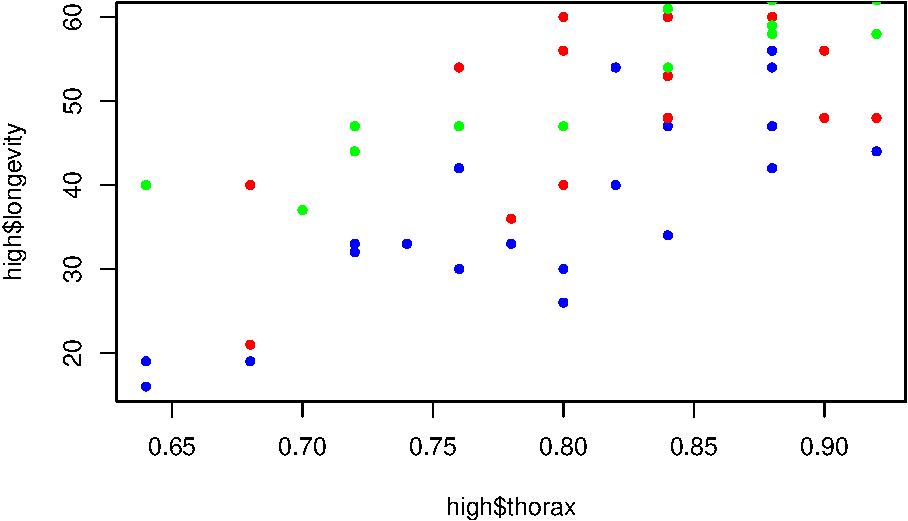
\includegraphics{Assignment2_complete_files/figure-latex/unnamed-chunk-28-1.pdf}
Here, we can see a clear increase in longevity when the thorax length
increases, for each of the three activity types. This indicates that the
the higher the thorax length, the higher the longevity. To check if this
is actually statistically significant for each of the three activity
types, we use a one-way ANOVA test for each of the activities:

\begin{Shaded}
\begin{Highlighting}[]
\NormalTok{high\_model }\OtherTok{\textless{}{-}} \FunctionTok{aov}\NormalTok{(loglongevity }\SpecialCharTok{\textasciitilde{}}\NormalTok{ thorax, }\AttributeTok{data=}\NormalTok{high)}
\FunctionTok{summary}\NormalTok{(high\_model)}
\end{Highlighting}
\end{Shaded}

\begin{verbatim}
##             Df Sum Sq Mean Sq F value   Pr(>F)    
## thorax       1 2.0760  2.0760   53.61 1.89e-07 ***
## Residuals   23 0.8906  0.0387                     
## ---
## Signif. codes:  0 '***' 0.001 '**' 0.01 '*' 0.05 '.' 0.1 ' ' 1
\end{verbatim}

\begin{Shaded}
\begin{Highlighting}[]
\FunctionTok{print}\NormalTok{(}\StringTok{\textquotesingle{}{-}{-}{-}{-}{-}{-}{-}{-}{-}{-}{-}{-}{-}{-}{-}{-}{-}{-}{-}{-}{-}{-}{-}{-}{-}{-}{-}{-}{-}{-}{-}{-}{-}{-}{-}{-}{-}{-}{-}{-}{-}{-}{-}\textquotesingle{}}\NormalTok{)}
\end{Highlighting}
\end{Shaded}

\begin{verbatim}
## [1] "-------------------------------------------"
\end{verbatim}

\begin{Shaded}
\begin{Highlighting}[]
\NormalTok{low\_model }\OtherTok{\textless{}{-}} \FunctionTok{aov}\NormalTok{(loglongevity }\SpecialCharTok{\textasciitilde{}}\NormalTok{ thorax, }\AttributeTok{data=}\NormalTok{low)}
\FunctionTok{summary}\NormalTok{(low\_model)}
\end{Highlighting}
\end{Shaded}

\begin{verbatim}
##             Df Sum Sq Mean Sq F value   Pr(>F)    
## thorax       1  1.006  1.0057   19.81 0.000183 ***
## Residuals   23  1.168  0.0508                     
## ---
## Signif. codes:  0 '***' 0.001 '**' 0.01 '*' 0.05 '.' 0.1 ' ' 1
\end{verbatim}

\begin{Shaded}
\begin{Highlighting}[]
\FunctionTok{print}\NormalTok{(}\StringTok{\textquotesingle{}{-}{-}{-}{-}{-}{-}{-}{-}{-}{-}{-}{-}{-}{-}{-}{-}{-}{-}{-}{-}{-}{-}{-}{-}{-}{-}{-}{-}{-}{-}{-}{-}{-}{-}{-}{-}{-}{-}{-}{-}{-}{-}{-}\textquotesingle{}}\NormalTok{)}
\end{Highlighting}
\end{Shaded}

\begin{verbatim}
## [1] "-------------------------------------------"
\end{verbatim}

\begin{Shaded}
\begin{Highlighting}[]
\NormalTok{isolated\_model }\OtherTok{\textless{}{-}} \FunctionTok{aov}\NormalTok{(loglongevity }\SpecialCharTok{\textasciitilde{}}\NormalTok{ thorax, }\AttributeTok{data=}\NormalTok{isolated)}
\FunctionTok{summary}\NormalTok{(isolated\_model)}
\end{Highlighting}
\end{Shaded}

\begin{verbatim}
##             Df Sum Sq Mean Sq F value   Pr(>F)    
## thorax       1 0.9511  0.9511      31 1.15e-05 ***
## Residuals   23 0.7055  0.0307                     
## ---
## Signif. codes:  0 '***' 0.001 '**' 0.01 '*' 0.05 '.' 0.1 ' ' 1
\end{verbatim}

In the results, we can see that the p-values for each activity type are
below 0.05. Therefore, the difference is statistically significant for
each activity type.

\hypertarget{d.}{%
\subsubsection{3d.}\label{d.}}

Since both the thorax length and the activity type influence the
longevity, we prefer the analysis with thorax length, as this is a more
complete analysis. However, since the thorax length influences the
longevity the same way for each activity type, the analysis without the
thorax length is still correct. If the thorax length would influence the
longevity differently for each activity type, then it would be incorrect
to analyse the data without the thorax length.

\hypertarget{e.}{%
\subsubsection{3e.}\label{e.}}

We now perform the ANCOVA analysis, but with the longevity as the
response variable instead of the log longevity:

\begin{Shaded}
\begin{Highlighting}[]
\NormalTok{fruitflies\_model2 }\OtherTok{=} \FunctionTok{drop1}\NormalTok{(}\FunctionTok{lm}\NormalTok{(longevity }\SpecialCharTok{\textasciitilde{}}\NormalTok{ activity }\SpecialCharTok{+}\NormalTok{ thorax, }\AttributeTok{data=}\NormalTok{fruitflies), }\AttributeTok{test=}\StringTok{"F"}\NormalTok{)}
\NormalTok{fruitflies\_model2}
\end{Highlighting}
\end{Shaded}

\begin{verbatim}
## Single term deletions
## 
## Model:
## longevity ~ activity + thorax
##          Df Sum of Sq   RSS    AIC F value    Pr(>F)    
## <none>                 7673 355.10                      
## activity  2    4966.7 12640 388.53  22.979 2.016e-08 ***
## thorax    1    7686.8 15360 405.15  71.127 2.624e-12 ***
## ---
## Signif. codes:  0 '***' 0.001 '**' 0.01 '*' 0.05 '.' 0.1 ' ' 1
\end{verbatim}

\begin{Shaded}
\begin{Highlighting}[]
\FunctionTok{summary}\NormalTok{(fruitflies\_model2)}
\end{Highlighting}
\end{Shaded}

\begin{verbatim}
##        Df         Sum of Sq         RSS             AIC           F value     
##  Min.   :1.00   Min.   :4967   Min.   : 7673   Min.   :355.1   Min.   :22.98  
##  1st Qu.:1.25   1st Qu.:5647   1st Qu.:10156   1st Qu.:371.8   1st Qu.:35.02  
##  Median :1.50   Median :6327   Median :12640   Median :388.5   Median :47.05  
##  Mean   :1.50   Mean   :6327   Mean   :11891   Mean   :382.9   Mean   :47.05  
##  3rd Qu.:1.75   3rd Qu.:7007   3rd Qu.:14000   3rd Qu.:396.8   3rd Qu.:59.09  
##  Max.   :2.00   Max.   :7687   Max.   :15360   Max.   :405.2   Max.   :71.13  
##  NA's   :1      NA's   :1                                      NA's   :1      
##      Pr(>F) 
##  Min.   :0  
##  1st Qu.:0  
##  Median :0  
##  Mean   :0  
##  3rd Qu.:0  
##  Max.   :0  
##  NA's   :1
\end{verbatim}

The p-values are still well below 0.05, so the results are still
statistically significant. However, the Sum Sq and Mean Sq values are
now so high that they are meaningless. Therefore, it is wise to use the
log longevity as the response variable and not the longevity.

\hypertarget{section-3}{%
\subsection{4}\label{section-3}}

PART a :

\begin{Shaded}
\begin{Highlighting}[]
\NormalTok{psidata }\OtherTok{\textless{}{-}} \FunctionTok{read.csv}\NormalTok{(}\StringTok{"psi.txt"}\NormalTok{, }\AttributeTok{sep=}\StringTok{""}\NormalTok{)}

\NormalTok{psidata}\SpecialCharTok{$}\NormalTok{gpa}\OtherTok{=}\FunctionTok{as.numeric}\NormalTok{(psidata}\SpecialCharTok{$}\NormalTok{gpa)}
\NormalTok{psidata}\SpecialCharTok{$}\NormalTok{psi}\OtherTok{=}\FunctionTok{as.factor}\NormalTok{(psidata}\SpecialCharTok{$}\NormalTok{psi)}
\FunctionTok{is.factor}\NormalTok{(psidata}\SpecialCharTok{$}\NormalTok{psi)}
\end{Highlighting}
\end{Shaded}

\begin{verbatim}
## [1] TRUE
\end{verbatim}

\begin{Shaded}
\begin{Highlighting}[]
\NormalTok{glm\_model}\OtherTok{=}\FunctionTok{glm}\NormalTok{(passed}\SpecialCharTok{\textasciitilde{}}\NormalTok{psi}\SpecialCharTok{*}\NormalTok{gpa,}\AttributeTok{data=}\NormalTok{psidata,}\AttributeTok{family=}\NormalTok{binomial)}
\FunctionTok{anova}\NormalTok{(glm\_model,}\AttributeTok{test=}\StringTok{"Chisq"}\NormalTok{) }\CommentTok{\# only the last p value is relevant}
\end{Highlighting}
\end{Shaded}

\begin{verbatim}
## Analysis of Deviance Table
## 
## Model: binomial, link: logit
## 
## Response: passed
## 
## Terms added sequentially (first to last)
## 
## 
##         Df Deviance Resid. Df Resid. Dev Pr(>Chi)   
## NULL                       31     41.183            
## psi      1   5.8418        30     35.342 0.015650 * 
## gpa      1   9.0885        29     26.253 0.002572 **
## psi:gpa  1   1.8725        28     24.381 0.171189   
## ---
## Signif. codes:  0 '***' 0.001 '**' 0.01 '*' 0.05 '.' 0.1 ' ' 1
\end{verbatim}

p-value of interaction between psi and gpa is greater than 0.05.
Therefore, the interaction is not significant between factor psi and
predictor grade.

\begin{Shaded}
\begin{Highlighting}[]
\NormalTok{glm2 }\OtherTok{=} \FunctionTok{glm}\NormalTok{(passed}\SpecialCharTok{\textasciitilde{}}\NormalTok{psi}\SpecialCharTok{+}\NormalTok{gpa,}\AttributeTok{data=}\NormalTok{psidata,}\AttributeTok{family=}\NormalTok{binomial)}
\FunctionTok{drop1}\NormalTok{(glm2,}\AttributeTok{test=}\StringTok{"Chisq"}\NormalTok{)}
\end{Highlighting}
\end{Shaded}

\begin{verbatim}
## Single term deletions
## 
## Model:
## passed ~ psi + gpa
##        Df Deviance    AIC    LRT Pr(>Chi)   
## <none>      26.253 32.253                   
## psi     1   32.418 36.418 6.1647 0.013033 * 
## gpa     1   35.342 39.342 9.0885 0.002572 **
## ---
## Signif. codes:  0 '***' 0.001 '**' 0.01 '*' 0.05 '.' 0.1 ' ' 1
\end{verbatim}

p-value for psi and gpa is less than 0.05. Therefore, they are
significant.

\begin{Shaded}
\begin{Highlighting}[]
\FunctionTok{summary}\NormalTok{(glm2)}
\end{Highlighting}
\end{Shaded}

\begin{verbatim}
## 
## Call:
## glm(formula = passed ~ psi + gpa, family = binomial, data = psidata)
## 
## Deviance Residuals: 
##     Min       1Q   Median       3Q      Max  
## -1.8396  -0.6282  -0.3045   0.5629   2.0378  
## 
## Coefficients:
##             Estimate Std. Error z value Pr(>|z|)   
## (Intercept)  -11.602      4.213  -2.754  0.00589 **
## psi1           2.338      1.041   2.246  0.02470 * 
## gpa            3.063      1.223   2.505  0.01224 * 
## ---
## Signif. codes:  0 '***' 0.001 '**' 0.01 '*' 0.05 '.' 0.1 ' ' 1
## 
## (Dispersion parameter for binomial family taken to be 1)
## 
##     Null deviance: 41.183  on 31  degrees of freedom
## Residual deviance: 26.253  on 29  degrees of freedom
## AIC: 32.253
## 
## Number of Fisher Scoring iterations: 5
\end{verbatim}

-11.602 + 2.338 + 3.063*x psi has a positive effect on probability of
success(i.e.~pass = 1). Therefore, it works. It increases the odds by
e\^{}2.338 = 10.36

\begin{Shaded}
\begin{Highlighting}[]
\FunctionTok{is.factor}\NormalTok{(psidata}\SpecialCharTok{$}\NormalTok{psi)}
\end{Highlighting}
\end{Shaded}

\begin{verbatim}
## [1] TRUE
\end{verbatim}

PART b:

\begin{Shaded}
\begin{Highlighting}[]
\NormalTok{newdata}\OtherTok{=}\FunctionTok{data.frame}\NormalTok{(}\AttributeTok{psi=}\DecValTok{1}\NormalTok{,}\AttributeTok{gpa=}\DecValTok{3}\NormalTok{)}
\NormalTok{newdata}\SpecialCharTok{$}\NormalTok{psi }\OtherTok{\textless{}{-}} \FunctionTok{as.factor}\NormalTok{(newdata}\SpecialCharTok{$}\NormalTok{psi)}
\FunctionTok{predict}\NormalTok{(glm2,newdata,}\AttributeTok{type=}\StringTok{"response"}\NormalTok{)}
\end{Highlighting}
\end{Shaded}

\begin{verbatim}
##         1 
## 0.4815864
\end{verbatim}

\begin{Shaded}
\begin{Highlighting}[]
\NormalTok{newdata2}\OtherTok{=}\FunctionTok{data.frame}\NormalTok{(}\AttributeTok{psi=}\DecValTok{0}\NormalTok{,}\AttributeTok{gpa=}\DecValTok{3}\NormalTok{)}
\NormalTok{newdata2}\SpecialCharTok{$}\NormalTok{psi }\OtherTok{\textless{}{-}} \FunctionTok{as.factor}\NormalTok{(newdata2}\SpecialCharTok{$}\NormalTok{psi)}
\FunctionTok{predict}\NormalTok{(glm2,newdata2,}\AttributeTok{type=}\StringTok{"response"}\NormalTok{)}
\end{Highlighting}
\end{Shaded}

\begin{verbatim}
##          1 
## 0.08230274
\end{verbatim}

Therefore, higher grade of 3 is more probable with psi than without psi.

PART c:

-11.602 + 2.338 + 3.063*x psi has a positive effect on probability of
success(i.e.~pass = 1). Therefore, it works. It increases the odds by
e\^{}2.338 = 10.36 Therefore, it increases the success probability(of
passing the exam) by 10 times with psi as compared to without psi.This
number is not depenedent on gpa.

PART d: CONTINGENCY TABLES: Check if psi and passed is independent or
not.

\begin{Shaded}
\begin{Highlighting}[]
\NormalTok{tot}\OtherTok{=}\FunctionTok{xtabs}\NormalTok{(}\SpecialCharTok{\textasciitilde{}}\NormalTok{psi}\SpecialCharTok{+}\NormalTok{passed,}\AttributeTok{data=}\NormalTok{psidata)}
\NormalTok{tot}
\end{Highlighting}
\end{Shaded}

\begin{verbatim}
##    passed
## psi  0  1
##   0 15  3
##   1  6  8
\end{verbatim}

\begin{Shaded}
\begin{Highlighting}[]
\NormalTok{z}\OtherTok{=}\FunctionTok{chisq.test}\NormalTok{(tot); z}
\end{Highlighting}
\end{Shaded}

\begin{verbatim}
## Warning in chisq.test(tot): Chi-squared approximation may be incorrect
\end{verbatim}

\begin{verbatim}
## 
##  Pearson's Chi-squared test with Yates' continuity correction
## 
## data:  tot
## X-squared = 4.0657, df = 1, p-value = 0.04376
\end{verbatim}

\begin{Shaded}
\begin{Highlighting}[]
\FunctionTok{chisq.test}\NormalTok{(tot,}\AttributeTok{simulate.p.value=}\ConstantTok{TRUE}\NormalTok{)}
\end{Highlighting}
\end{Shaded}

\begin{verbatim}
## 
##  Pearson's Chi-squared test with simulated p-value (based on 2000
##  replicates)
## 
## data:  tot
## X-squared = 5.7192, df = NA, p-value = 0.02599
\end{verbatim}

they are not independent as p-value is less than 0.05. Therefore, passed
and psi are dependent.

It is a 2*2 table, therefore we can also use fischer's exact test. From
this test we can get the exact p-value.

\begin{Shaded}
\begin{Highlighting}[]
\FunctionTok{fisher.test}\NormalTok{(tot)}
\end{Highlighting}
\end{Shaded}

\begin{verbatim}
## 
##  Fisher's Exact Test for Count Data
## 
## data:  tot
## p-value = 0.0265
## alternative hypothesis: true odds ratio is not equal to 1
## 95 percent confidence interval:
##   1.047057 49.595860
## sample estimates:
## odds ratio 
##   6.227408
\end{verbatim}

Therefore, exact p-value is 0.0265. Fischer test approach is valid here.

\begin{Shaded}
\begin{Highlighting}[]
\NormalTok{ratio }\OtherTok{=}\NormalTok{ (}\DecValTok{6}\SpecialCharTok{/}\DecValTok{15}\NormalTok{)}\SpecialCharTok{/}\NormalTok{(}\DecValTok{8}\SpecialCharTok{/}\DecValTok{3}\NormalTok{)}
\FunctionTok{print}\NormalTok{(ratio)}
\end{Highlighting}
\end{Shaded}

\begin{verbatim}
## [1] 0.15
\end{verbatim}

For every one student with psi and who has passed there is 0.15 that
failed.

PART e:

Fischer test approach is valid here.

Advantage of logistic but disadvantage of contingency table : By second
approach, we show there is dependency but it doesn't quanitfy it.
Whereas we can numerically express the relation between psi and passed
from logistic regression. We can't make predictions with the results of
the fisher's exact test.

Fischer test is more suited for small sample size.

Advantage of contigency but disadvantage of logistic

\hypertarget{section-4}{%
\subsection{5}\label{section-4}}

Load awards.txt

\begin{Shaded}
\begin{Highlighting}[]
\NormalTok{awards }\OtherTok{=} \FunctionTok{read.csv}\NormalTok{(}\StringTok{"awards.txt"}\NormalTok{, }\AttributeTok{sep=}\StringTok{""}\NormalTok{)}
\end{Highlighting}
\end{Shaded}

\hypertarget{a.-2}{%
\subsubsection{5a.}\label{a.-2}}

We perform Poisson regression using the variable program

\begin{Shaded}
\begin{Highlighting}[]
\NormalTok{poisson\_awards }\OtherTok{\textless{}{-}} \FunctionTok{glm}\NormalTok{(num\_awards }\SpecialCharTok{\textasciitilde{}}\NormalTok{ prog, }\AttributeTok{family=}\StringTok{"poisson"}\NormalTok{, }\AttributeTok{data=}\NormalTok{awards)}
\CommentTok{\#poisson\_awards}
\FunctionTok{summary}\NormalTok{(poisson\_awards)}
\end{Highlighting}
\end{Shaded}

\begin{verbatim}
## 
## Call:
## glm(formula = num_awards ~ prog, family = "poisson", data = awards)
## 
## Deviance Residuals: 
##     Min       1Q   Median       3Q      Max  
## -1.4974  -1.2833  -0.1165   0.1881   3.4500  
## 
## Coefficients:
##             Estimate Std. Error z value Pr(>|z|)
## (Intercept)  -0.3485     0.2311  -1.508    0.131
## prog          0.1543     0.1047   1.474    0.141
## 
## (Dispersion parameter for poisson family taken to be 1)
## 
##     Null deviance: 228.83  on 199  degrees of freedom
## Residual deviance: 226.65  on 198  degrees of freedom
## AIC: 520.97
## 
## Number of Fisher Scoring iterations: 5
\end{verbatim}

Here, the p-value is greater than 0.05, so the variable program alone
does not influence the number of awards.

Next, we estimate the number of awards of each type of program,
according to the Poisson model. We create new dataframes that contain
each of the program type, and use the predict() function to apply the
model to the awards type.

\begin{Shaded}
\begin{Highlighting}[]
\NormalTok{new\_data }\OtherTok{=} \FunctionTok{data.frame}\NormalTok{(}\AttributeTok{prog=}\DecValTok{1}\NormalTok{)}
\FunctionTok{predict}\NormalTok{(poisson\_awards, }\AttributeTok{newdata=}\NormalTok{new\_data, }\AttributeTok{type =} \StringTok{"response"}\NormalTok{)}
\end{Highlighting}
\end{Shaded}

\begin{verbatim}
##         1 
## 0.8234681
\end{verbatim}

\begin{Shaded}
\begin{Highlighting}[]
\NormalTok{new\_data }\OtherTok{=} \FunctionTok{data.frame}\NormalTok{(}\AttributeTok{prog=}\DecValTok{2}\NormalTok{)}
\FunctionTok{predict}\NormalTok{(poisson\_awards, }\AttributeTok{newdata=}\NormalTok{new\_data, }\AttributeTok{type =} \StringTok{"response"}\NormalTok{)}
\end{Highlighting}
\end{Shaded}

\begin{verbatim}
##         1 
## 0.9608369
\end{verbatim}

\begin{Shaded}
\begin{Highlighting}[]
\NormalTok{new\_data }\OtherTok{=} \FunctionTok{data.frame}\NormalTok{(}\AttributeTok{prog=}\DecValTok{3}\NormalTok{)}
\FunctionTok{predict}\NormalTok{(poisson\_awards, }\AttributeTok{newdata=}\NormalTok{new\_data, }\AttributeTok{type =} \StringTok{"response"}\NormalTok{)}
\end{Highlighting}
\end{Shaded}

\begin{verbatim}
##        1 
## 1.121121
\end{verbatim}

According to the results, program \emph{academic} (3) results in the
highest number of awards, which is 1.12.

\hypertarget{b.-2}{%
\subsubsection{5b.}\label{b.-2}}

\begin{Shaded}
\begin{Highlighting}[]
\NormalTok{prog1 }\OtherTok{=} \FunctionTok{subset}\NormalTok{(awards, prog}\SpecialCharTok{==}\DecValTok{1}\NormalTok{)}
\FunctionTok{hist}\NormalTok{(prog1}\SpecialCharTok{$}\NormalTok{num\_awards)}
\end{Highlighting}
\end{Shaded}

\includegraphics{Assignment2_complete_files/figure-latex/unnamed-chunk-43-1.pdf}

\begin{Shaded}
\begin{Highlighting}[]
\NormalTok{prog2 }\OtherTok{=} \FunctionTok{subset}\NormalTok{(awards, prog}\SpecialCharTok{==}\DecValTok{2}\NormalTok{)}
\FunctionTok{hist}\NormalTok{(prog2}\SpecialCharTok{$}\NormalTok{num\_awards)}
\end{Highlighting}
\end{Shaded}

\includegraphics{Assignment2_complete_files/figure-latex/unnamed-chunk-43-2.pdf}

\begin{Shaded}
\begin{Highlighting}[]
\NormalTok{prog3 }\OtherTok{=} \FunctionTok{subset}\NormalTok{(awards, prog}\SpecialCharTok{==}\DecValTok{3}\NormalTok{)}
\FunctionTok{hist}\NormalTok{(prog3}\SpecialCharTok{$}\NormalTok{num\_awards)}
\end{Highlighting}
\end{Shaded}

\includegraphics{Assignment2_complete_files/figure-latex/unnamed-chunk-43-3.pdf}
The distributions have the same shape, the response variable is ordinal
and we assume independence. Therefore, we \emph{can} apply the
Kruskal-Wallis test. Performing this test:

\begin{Shaded}
\begin{Highlighting}[]
\NormalTok{kruskal\_wallis}\OtherTok{\textless{}{-}}\FunctionTok{kruskal.test}\NormalTok{(num\_awards }\SpecialCharTok{\textasciitilde{}}\NormalTok{ prog, }\AttributeTok{data=}\NormalTok{awards)}
\NormalTok{kruskal\_wallis}
\end{Highlighting}
\end{Shaded}

\begin{verbatim}
## 
##  Kruskal-Wallis rank sum test
## 
## data:  num_awards by prog
## Kruskal-Wallis chi-squared = 10.755, df = 2, p-value = 0.00462
\end{verbatim}

Here, the p-value is lower than 0.05, which implies that the program
\emph{does} influence the number of awards.

\hypertarget{c-1}{%
\subsubsection{5c}\label{c-1}}

We perform Poisson regression using both the variables math and program:

\begin{Shaded}
\begin{Highlighting}[]
\NormalTok{poisson\_awards }\OtherTok{\textless{}{-}} \FunctionTok{glm}\NormalTok{(num\_awards }\SpecialCharTok{\textasciitilde{}}\NormalTok{ prog}\SpecialCharTok{+}\NormalTok{math, }\AttributeTok{family=}\StringTok{"poisson"}\NormalTok{, }\AttributeTok{data=}\NormalTok{awards)}
\CommentTok{\#poisson\_awards}
\FunctionTok{summary}\NormalTok{(poisson\_awards)}
\end{Highlighting}
\end{Shaded}

\begin{verbatim}
## 
## Call:
## glm(formula = num_awards ~ prog + math, family = "poisson", data = awards)
## 
## Deviance Residuals: 
##      Min        1Q    Median        3Q       Max  
## -1.98567  -1.14535  -0.05993   0.33887   2.55070  
## 
## Coefficients:
##              Estimate Std. Error z value Pr(>|z|)    
## (Intercept) -2.721628   0.524702  -5.187 2.14e-07 ***
## prog         0.263565   0.117082   2.251   0.0244 *  
## math         0.039541   0.007455   5.304 1.13e-07 ***
## ---
## Signif. codes:  0 '***' 0.001 '**' 0.01 '*' 0.05 '.' 0.1 ' ' 1
## 
## (Dispersion parameter for poisson family taken to be 1)
## 
##     Null deviance: 228.83  on 199  degrees of freedom
## Residual deviance: 199.08  on 197  degrees of freedom
## AIC: 495.4
## 
## Number of Fisher Scoring iterations: 5
\end{verbatim}

When using math and program, the p-values for both variables are below
0.05, and are thus significant. This is interesting, as creating the
model using only the program variable yields that program is not
significant in influencing the number of awards. This means that the
model using only the program variable is insufficient.

To see which program is most effective, we use the model to predict the
number of awards for each program, using both the maximum and minimum
values of the math variable

\begin{Shaded}
\begin{Highlighting}[]
\FunctionTok{print}\NormalTok{(}\StringTok{"Program 1"}\NormalTok{)}
\end{Highlighting}
\end{Shaded}

\begin{verbatim}
## [1] "Program 1"
\end{verbatim}

\begin{Shaded}
\begin{Highlighting}[]
\NormalTok{new\_data }\OtherTok{=} \FunctionTok{data.frame}\NormalTok{(}\AttributeTok{prog=}\DecValTok{1}\NormalTok{, }\AttributeTok{math=}\FunctionTok{max}\NormalTok{(awards}\SpecialCharTok{$}\NormalTok{math))}
\FunctionTok{predict}\NormalTok{(poisson\_awards, }\AttributeTok{newdata=}\NormalTok{new\_data, }\AttributeTok{type =} \StringTok{"response"}\NormalTok{)}
\end{Highlighting}
\end{Shaded}

\begin{verbatim}
##        1 
## 1.661149
\end{verbatim}

\begin{Shaded}
\begin{Highlighting}[]
\NormalTok{new\_data }\OtherTok{=} \FunctionTok{data.frame}\NormalTok{(}\AttributeTok{prog=}\DecValTok{1}\NormalTok{, }\AttributeTok{math=}\FunctionTok{min}\NormalTok{(awards}\SpecialCharTok{$}\NormalTok{math))}
\FunctionTok{predict}\NormalTok{(poisson\_awards, }\AttributeTok{newdata=}\NormalTok{new\_data, }\AttributeTok{type =} \StringTok{"response"}\NormalTok{)}
\end{Highlighting}
\end{Shaded}

\begin{verbatim}
##         1 
## 0.3156216
\end{verbatim}

\begin{Shaded}
\begin{Highlighting}[]
\FunctionTok{print}\NormalTok{(}\StringTok{"Program 2"}\NormalTok{)}
\end{Highlighting}
\end{Shaded}

\begin{verbatim}
## [1] "Program 2"
\end{verbatim}

\begin{Shaded}
\begin{Highlighting}[]
\NormalTok{new\_data }\OtherTok{=} \FunctionTok{data.frame}\NormalTok{(}\AttributeTok{prog=}\DecValTok{2}\NormalTok{, }\AttributeTok{math=}\FunctionTok{max}\NormalTok{(awards}\SpecialCharTok{$}\NormalTok{math))}
\FunctionTok{predict}\NormalTok{(poisson\_awards, }\AttributeTok{newdata=}\NormalTok{new\_data, }\AttributeTok{type =} \StringTok{"response"}\NormalTok{)}
\end{Highlighting}
\end{Shaded}

\begin{verbatim}
##        1 
## 2.162087
\end{verbatim}

\begin{Shaded}
\begin{Highlighting}[]
\NormalTok{new\_data }\OtherTok{=} \FunctionTok{data.frame}\NormalTok{(}\AttributeTok{prog=}\DecValTok{2}\NormalTok{, }\AttributeTok{math=}\FunctionTok{min}\NormalTok{(awards}\SpecialCharTok{$}\NormalTok{math))}
\FunctionTok{predict}\NormalTok{(poisson\_awards, }\AttributeTok{newdata=}\NormalTok{new\_data, }\AttributeTok{type =} \StringTok{"response"}\NormalTok{)}
\end{Highlighting}
\end{Shaded}

\begin{verbatim}
##         1 
## 0.4108009
\end{verbatim}

\begin{Shaded}
\begin{Highlighting}[]
\FunctionTok{print}\NormalTok{(}\StringTok{"Program 3"}\NormalTok{)}
\end{Highlighting}
\end{Shaded}

\begin{verbatim}
## [1] "Program 3"
\end{verbatim}

\begin{Shaded}
\begin{Highlighting}[]
\NormalTok{new\_data }\OtherTok{=} \FunctionTok{data.frame}\NormalTok{(}\AttributeTok{prog=}\DecValTok{3}\NormalTok{, }\AttributeTok{math=}\FunctionTok{max}\NormalTok{(awards}\SpecialCharTok{$}\NormalTok{math))}
\FunctionTok{predict}\NormalTok{(poisson\_awards, }\AttributeTok{newdata=}\NormalTok{new\_data, }\AttributeTok{type =} \StringTok{"response"}\NormalTok{)}
\end{Highlighting}
\end{Shaded}

\begin{verbatim}
##       1 
## 2.81409
\end{verbatim}

\begin{Shaded}
\begin{Highlighting}[]
\NormalTok{new\_data }\OtherTok{=} \FunctionTok{data.frame}\NormalTok{(}\AttributeTok{prog=}\DecValTok{3}\NormalTok{, }\AttributeTok{math=}\FunctionTok{min}\NormalTok{(awards}\SpecialCharTok{$}\NormalTok{math))}
\FunctionTok{predict}\NormalTok{(poisson\_awards, }\AttributeTok{newdata=}\NormalTok{new\_data, }\AttributeTok{type =} \StringTok{"response"}\NormalTok{)}
\end{Highlighting}
\end{Shaded}

\begin{verbatim}
##         1 
## 0.5346826
\end{verbatim}

In the results, we can see that for both the maximum and minimum values
of the math variable, the number of awards is the highest for program 3.
Therefore program 3 is three is the best for the number of awards.

The number of awards for the vocational program (1) and the math score
of 55 is estimated by:

\begin{Shaded}
\begin{Highlighting}[]
\NormalTok{new\_data }\OtherTok{=} \FunctionTok{data.frame}\NormalTok{(}\AttributeTok{prog=}\DecValTok{1}\NormalTok{, }\AttributeTok{math=}\DecValTok{55}\NormalTok{)}
\FunctionTok{predict}\NormalTok{(poisson\_awards, }\AttributeTok{newdata=}\NormalTok{new\_data, }\AttributeTok{type =} \StringTok{"response"}\NormalTok{)}
\end{Highlighting}
\end{Shaded}

\begin{verbatim}
##         1 
## 0.7532863
\end{verbatim}

Thus, the number of awards for the vocational program and math score 55
is 0.75.

\end{document}
